%!TEX root = ../../main.tex
\subsection{Station Software}\label{subsec:stationsoftdesfgi}
While \figref{fig:overallarch} of the overall architecture provides an overview of the system, the station component has its own architecture as well, which can be seen in \figref{fig:stationarch}. In this figure, as in the previous, the arrows represent flow of information.

\begin{figure}[h]
	\centering
	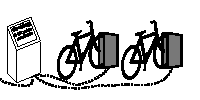
\includegraphics[trim=2cm 9.5cm 0cm 3cm, clip, scale=0.7]{design/station}
	\caption{Station software architecture.}\label{fig:stationarch}
\end{figure}

In the station software, the station is the main part and also the one that contains the UI. 
This part is responsible for all contact with the user at the station and is the one that is interacting with the hardware.

\texttt{TCPListener} is a thread that listens for messages from the global system through the \texttt{Website\-ToStationNotifier} and stores these messages as a \texttt{NetworkData} object, and tells this object to perform the action the message contains.

The \texttt{NetworkData} object has the responsibility of adding a booking to the local database corresponding to the information the object contains or removing a booking with the ID it received.

The \texttt{LockManager} is also a thread, and is responsible for locking a bicycle when a booking is close to its start time and unlocking said bicycle again if the booking's start time is exceeded by a certain limit.

The last class is the \texttt{ServiceThreads} which is also running in a separate thread.
This thread is responsible for reporting changes at the station, which are stored in the \texttt{ActionQueue} queue.
As soon as there is something in the \texttt{ActionQueue} queue, the thread will try to report it to the online interface, repeating until it succeeds in transmitting it.

However, how locking should be tackled has not been touched upon yet, but is a  central part of the system and as of such is examined hereafter.

\subsubsection{Locking Considerations}\label{subsec:lockingcons}
Consider the scenario where a user $u_1$ makes a booking $b_1$ on the website at time $t_1$ wanting to reserve a bicycle for time $t_3$. Before time $t_1$ another user $u_2$ made a booking $b_2$ of a bicycle for time $t_2$. Both users made a booking at the same station, and the amount of available bicycles for that station was for both users 1. Under the assumption that a bicycle cannot be locked and thereby reserved before some amount of time, say $t_{before}$, before usage, this scenario is possible in the following way.

First consider this definition of a time $t$, it is a time represented as the number of seconds from Thursday, 1 January 1970 at 00:00:00 UTC, which is the Epoch time, as of such comparisons such as $>$ is just computed as usual on numbers.
Let, 
$$TSB(b) = \{(t_1,t_2) \;| \;t_1 = st(b) - t_{before} \land t_2 = st(b) \land t_1 \leq t_2 \}$$
where,
\begin{itemize}[align = left]
	\item[$st(b)$] is defined as the start time of booking $b$.
	\item[$TSB(b)$] defines the Time Span Before of booking $b$.
\end{itemize} 

\begin{figure}[h]
	\centering
	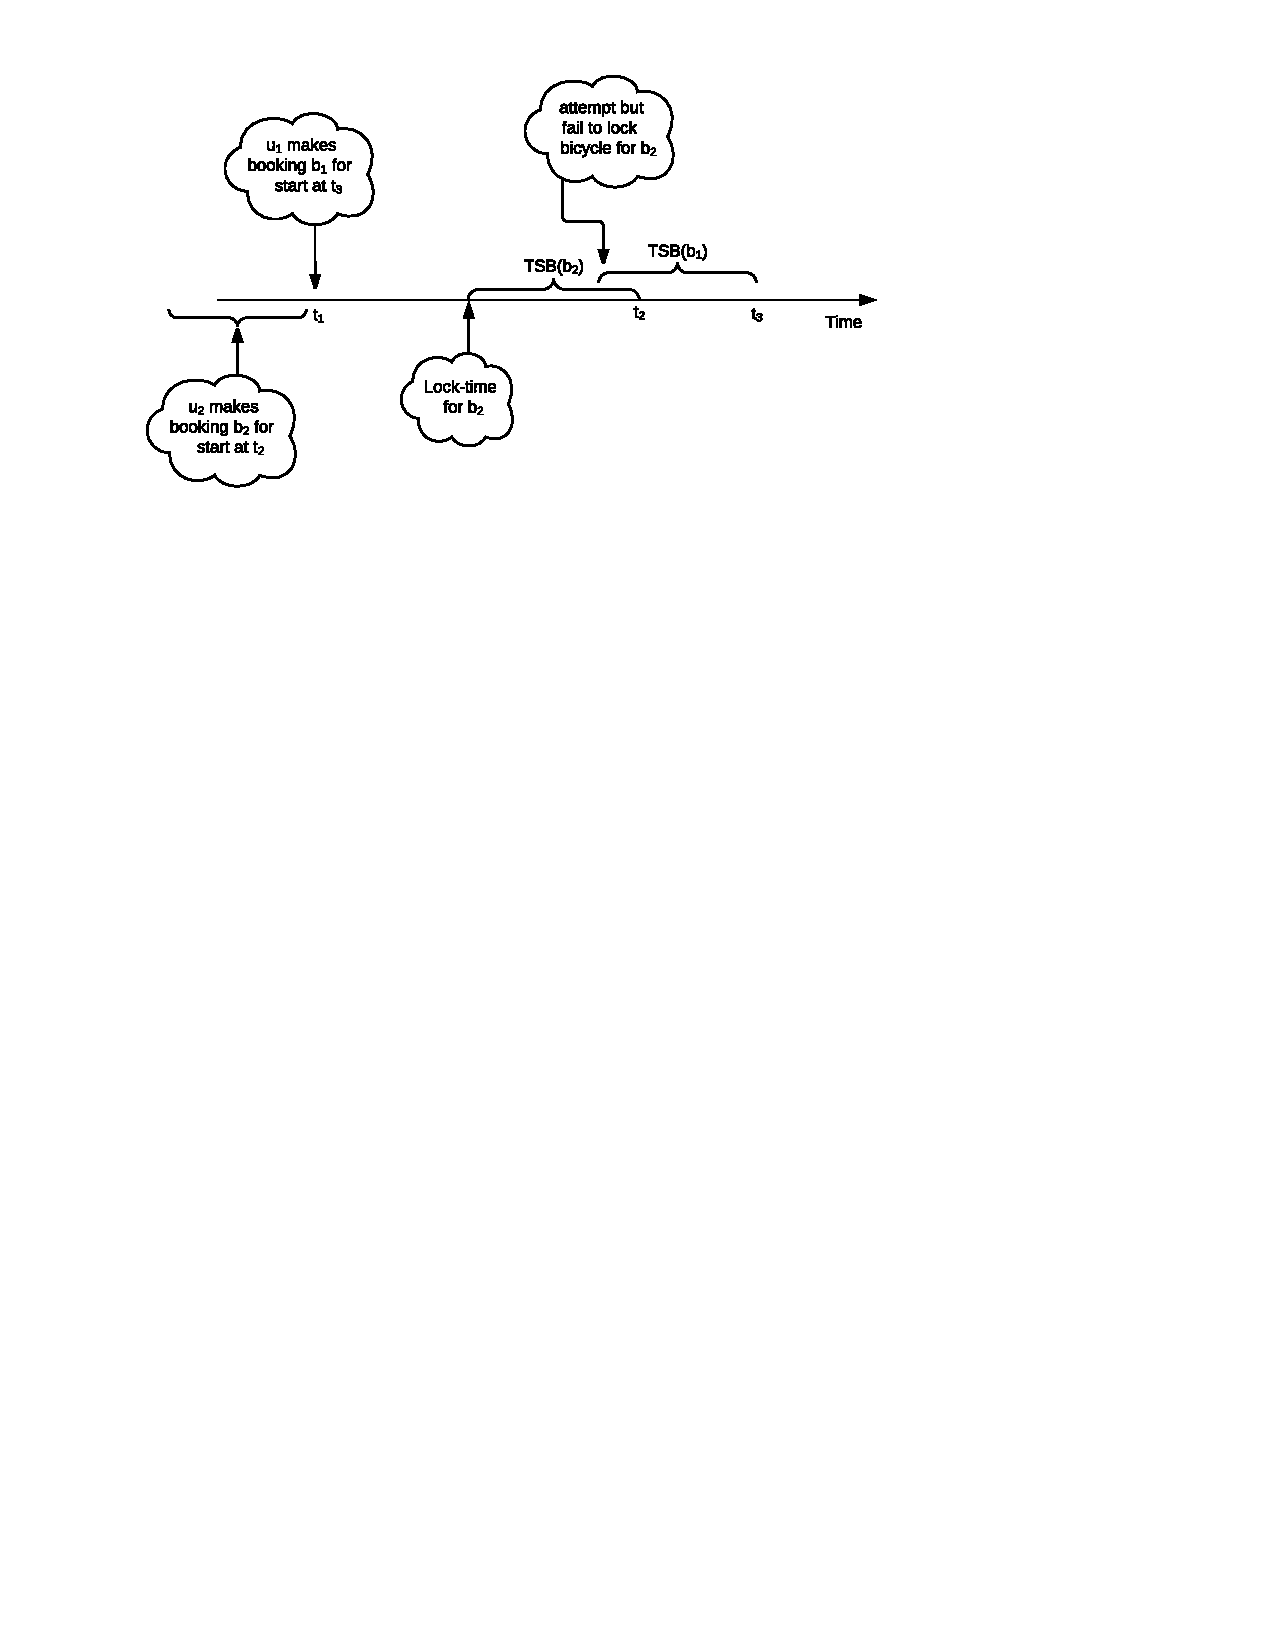
\includegraphics[trim = 1cm 19.7cm 0cm 0cm,clip]{behaviour/booking-illustration}
	\caption{Booking scenario illustration.}\label{fig:booking-illustartion}
\end{figure}
Then the scenario is given if $TSB(b_2)$ starts before $TSB(b_1)$ and $TSB(b_2)$ starts after $t_1$, we have a situation as can be seen in \figref{fig:booking-illustartion}.
As can be examined from the illustration, a problem occurs, under the assumption that no new bicycles gets delivered or taken from the given station in the given time-line, and where the amount of available bicycles before the lock-time of $b_2$ is 1.

The problem for user $u_1$ is then at time $t_1$ it appeared that a bicycle was available, but the bicycle is locked for user $u_2$ before it is locked for $u_1$ resulting in an availability count of 0 for $b_1$, thereby having no bicycle to lock for $u_1$.

The key aspect of why the handling of locking cannot be left as a responsibility of the database is to make the system less static, as requested by Aalborg Kommune, see \secref{subsec:meetingaalborg}.
If we were to make this a responsibility of the database, it would be in the case where locking should be performed immediately, but if you book a bicycle for tomorrow that would mean a bicycle would be unavailable for other users for a whole day, which is highly undesired.
An alternative would be to limit the time in advance you can make a booking, this would also increase the dynamic of the system, but would limit the booking flexibility.
This is a trade off between certainty of getting the bicycle booked and a dynamic system where more bicycles are in use.